\section{Results}
In the following, we present an evaluation of the predictors discussed in section \cref{sec:metadata}. 

\begin{table}
\centering
\begin{tabular}{| l | *{5}{c|}}
																				\cline{1-2}
valet		& 1																\\	\cline{1-3}
serviteur	& 0.367	& 1 													\\	\cline{1-4}
domestique	& 0.116	& 0.072 	& 1											\\	\cline{1-5}
p\^atissier	& 0.148	& 0.087		& 0.087			& 1							\\ 	\cline{1-6}
cuisinier 	& 0.211	& 0.156 	& 0.078			& 0.567			& 1			\\	\hline
 			& valet &serviteur	& domestique	&p\^atissier	& cuisiner	\\	\hline
\end{tabular}
\caption{Cosine distance for given word vectors using pre-trained word2vec model, with skip-gram architecture and dim=700.}
\label{tab:word_sim}
\end{table}

\subsection{Profession predictor}
In order to evaluate the precision of this predictor, we decided on utilizing the numerical representations of word embeddings to get a measure out of it, since the multiple possible outcomes made it impossible to qualify it as a classification. We wanted to be able to take semantic similarity into account. Word embeddings can provide this, to a certain extent. 

The pre-computed model we use is trained using the skip-gram model, which performs better than a continuous bag-of-words model for semantic similarities \cite{mikolov2013efficient}. The vectors are 700-dimensional and were computed on 1.6 billion words from French web domains

In effect this means we're able to get a numeric similarity between two words (or job-titles) by getting the cosine distance between their vector representations. We compare an extracted title with our hand-labeled title, and thus get a similarity score. This measure should be taken with a pinch of salt however, since the similarities weren't extensively tested on our job corpus. In \cref{tab:word_sim}, we see that the two highest scores are for the pairs `valet'-`serviteur' and `cuisinier'-`p\^atissier', which is as one would expect. However `domestique' has a surprisingly low similarity with both `valet' and `serviteur', which are semantically similar. Since the model uses PoS tags (i.e. `domestique\_n' to indicate it's a noun) to avoid ambiguity, this isn't due to confusion with its adjective form.

\begin{figure}
\centering
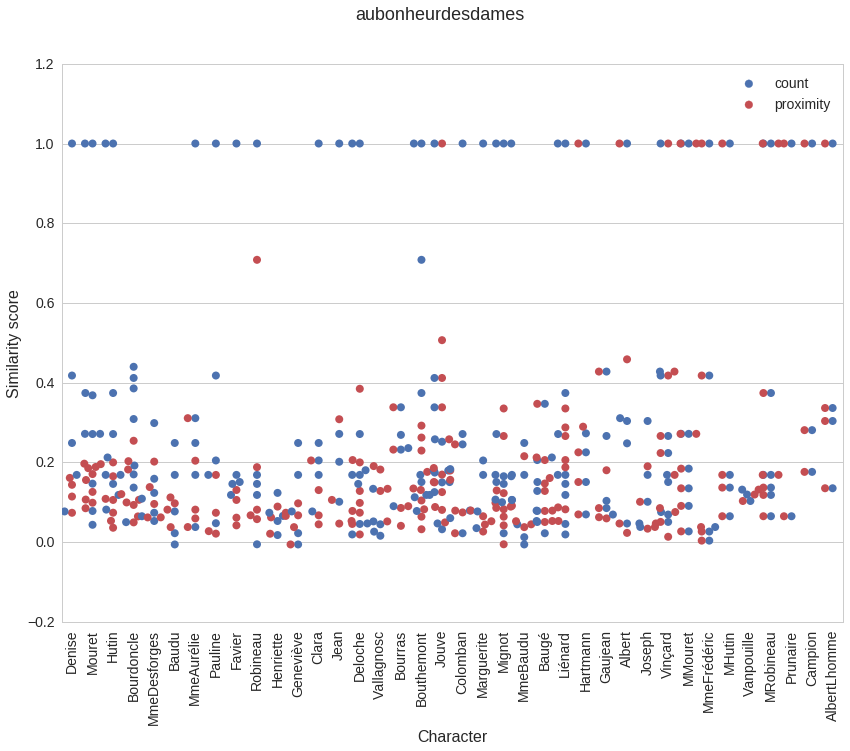
\includegraphics[width=.8\textwidth]{fig/count_vs_prox_bonheur.png}
\caption{Count vs Proximity predictor scores on \textit{Au Bonheur des Dames} characters. Points with score 1 are an exact match between two words. Characters are ordered by decreasing occurrence count. \textit{Note}: plots for other books are generally similar.}
\label{fig:count_vs_prox}
\end{figure}

The job predictor returns the 5 top guesses for a $c_i$'s job. In \cref{fig:count_vs_prox}, we show the result of the `count' and `proximity' predictors. In some cases, the job labels for the characters contain more than one possibility, which is why some characters have more points in the graph than others. The figure shows that the `count' predictor is far more present in the exact matches with the label, and `proximity' points are more pertinent when used for more minor characters. 

\begin{table}
\centering
\begin{tabular}{| l | *{5}{c|}}
\hline
& \multicolumn{5}{ |c| }{Rank} \\ \cline{2-6}
					& 0		& 1 	&2 		& 3		& 4		\\ \hline 
Individual ratio	& \textbf{0.41}	& 0.22	& 0.1	& 0.09	& 0.05	\\ \hline
Cumulative ratio	& 0.41	& 0.55	& 0.61	& 0.68	& 0.71	\\ \hline

\end{tabular}
\caption{Perfect match ratio for different ranks. The full character-set has 108 characters. The individual ratio is the ratio for only the given rank, and the cumulative is the ratio up until and including the given rank.}
\label{tab:match_ratio}
\end{table}

The results in \cref{fig:count_vs_prox} are encouraging, seeing as a majority of the characters (in this book, but also others) have an exact match between one its job-labels and at least one among the top 5 predictions. As an additional step, we look at the percentage of characters with exact matches in each of the 5 ranks in \cref{tab:match_ratio}. These were achieved using the `aggregate' predictor on the full book, with constant increments (c.f. figures below).

\begin{figure}
\centering
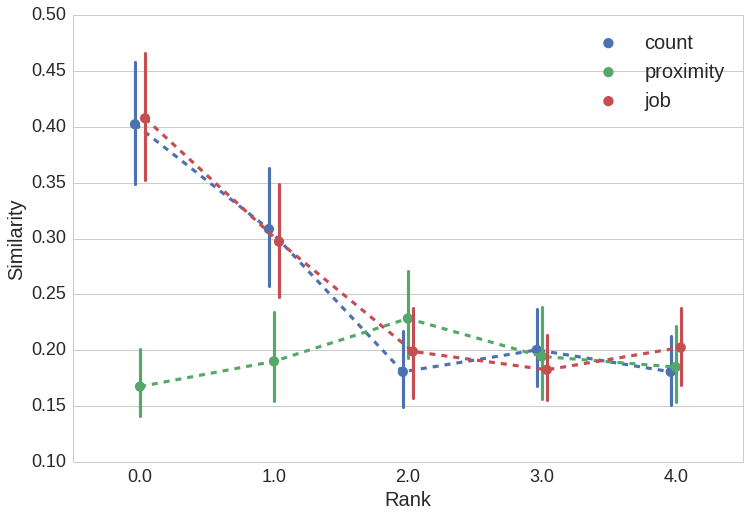
\includegraphics[width=.6\textwidth]{fig/rank_cpa.png}
\caption{Mean of all book and character scores grouped by 'rank' of prediction. Here the plots are of the `count', `proximity' and `aggregate' (first two combined) predictors. The bars represent the confidence interval for the point estimate.}
\label{fig:rank_cpa}
\end{figure}

To get an understanding of how the different guesses perform, in order, we plot the mean of all similarity scores (all books, all characters) grouped by the rank they were predicted in, in \cref{fig:rank_cpa}. The `aggregate' predictor is a combination of the other two, but with a higher weight given to the `count' predictor. We can see that it scores slightly higher than the `count' predictor for its first predictions.

\begin{figure}
\centering
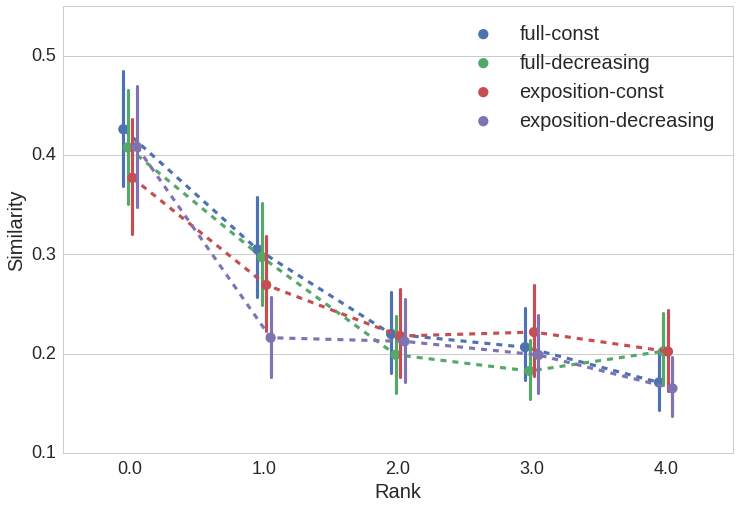
\includegraphics[width=.6\textwidth]{fig/job_params.png}
\caption{A comparison of the different parameters for the job predictor. `full' indicates the prediction was made based on observations from the whole book, whereas `exposition' focuses only on the $k$ first occurrences (here $\max(\frac{1}{10}L_i, 10)$, where $L_i$ is the length of $c_i$'s document). `decreasing' indicates that the weight of the contributions of each occurrence decreases (by rate seen in \cref{sec:metadata}) with occurrences later in $c_i$'s document.}
\label{fig:job_params}
\end{figure}

The effect of the different parameters of the job predictor are shown in \cref{fig:job_params}. We can see that the best similarity score on rank 0 and 1 is achieved with the `full-constant' parameter, but for ranks 2, 3 and 4 it's the `exposition-constant' that is on top. It seems working with the full range of data available in a characters document is generally preferable.

Both \cref{fig:rank_cpa} and \cref{fig:job_params} were created with approx 3000 data points, split evenly between the 5 `rank' categories. There are 108 distinct characters among them, taken from the 5 different books described in \cref{ssec:data}. Given the limited nature of this data, we should take the results presented above as indicators, but not entirely deterministic. The precision of these evaluations would benefit from more labeled books, and a system of expert reviewers for the labels.

The results above seem to work in favour of hypotheses 1 and 2 discussed in \cref{sec:metadata}. On the one hand, the result is slightly better when using a proximity score, and we also work with a constrained window size (maximum 5 sentences, with character occurrence at center), which performs better than larger sizes. This indicates there is an information gain from looking at and weighting the data close to the character higher, as hypothesis 1 stipulates. 

On the other, the predictor using only `exposition' occurrences (initial $\frac{1}{10}$th of total) has a performance very close to that of the `full' occurrences. Given that these occurrences are much fewer in number, and thus provide much less data overall, one can see that a lot of the metadata we're looking for will presumably be found within an exposition phase, as hypothesis 2 stipulates (first $k$ occurrences is called the `exposition' here).

\subsection{Gender predictor}
The evaluation of the gender predictor is more straightforward, since it is taken as a 2-class classification, i.e. we want to predict when a character is female. All characters were labeled with either a `m' (for male), `f' (for female) or `-' (for unknown) tag. The latter was given in cases where there wasn't a clear answer, for example when the predicted character name was used interchangeably for different family members (mother, father, children), or for animals of unknown gender. These characters were ignored in the classification metrics given below.

We provide the results for different feature generation schemes that we used, i.e. either all character $c_i$'s occurrences are taken, or only the ones where $c_i$ appears alone (filtered document). The accuracy, precision, recall and f-score metrics are shown in \cref{tab:gender_metrics}. Overall, the best performance is achieved when using the weighted features from the whole character documents. This is by a small margin however, so can't be considered conclusive. In part this is due to the greedy labeling of the name-gender predictor, since without it, there is a bigger gap in the ratio of guessed data points (approx. $7\%$) between the `solo' and `full' data. 

This failing of the `solo' data seems to be an argument against our 3rd hypothesis in \cref{sec:metadata}, but can also be attributed to the fewness of data in our character documents, and the general nature of the extracted features (i.e. only small percentage of sentences will get positive or negative score off these features).

\begin{table}
\centering
\begin{tabular}{| >{\bf}l || *{5}{c|}}
\hline
					& Accuracy & Precision	& Recall & F-score & Known ratio	\\ \hline \hline
GFNW	& 0.873 & 0.758 & 0.979	& 0.854	& 0.83 	\\ \hline
GSNW	& 0.878	& 0.793	& 0.938	& 0.859	& 0.81	\\ \hline
GFW		& 0.88	& 0.767	& 0.978	& 0.859	& 0.83 \\ \hline
GSW		& 0.869	& 0.779 & 0.938 & 0.851	& 0.81 \\ \hline

\end{tabular}
\caption{Comparison of different features and weights used on the gender prediction task.`G' is for gender, `F' means we used the full data, as opposed to `S' (for solo), where we worked only with sentences where the character occurs alone. `NW' means the scores are non-weighted, and `W' means they are weighted, with weights approximated from a logistic regression. The column 'Known ratio' indicates the ratio of data points for which the predictor was able to make a guess.}
\label{tab:gender_metrics}
\end{table}

We show the distribution of predicted and true labels in \cref{fig:gender}.
Interestingly, we see in \cref{fig:gender_dist} that the predictor tends to output more `female' labels than there are true data points of that category, and the opposite for the `male' category. We remarked on the problematic case of the neutral `il' in \cref{sssec:gender}. These results show that the bias even tends towards the opposite direction. This can be attributed to the efficiency of the multi-feature predictor, in that each feature contributes only a fraction of the result score. Additionally, the pronoun feature was shown to be less efficient and thus given a smaller weight than the other features. 

\begin{figure}
\centering
\begin{subfigure}[b]{0.45\textwidth}
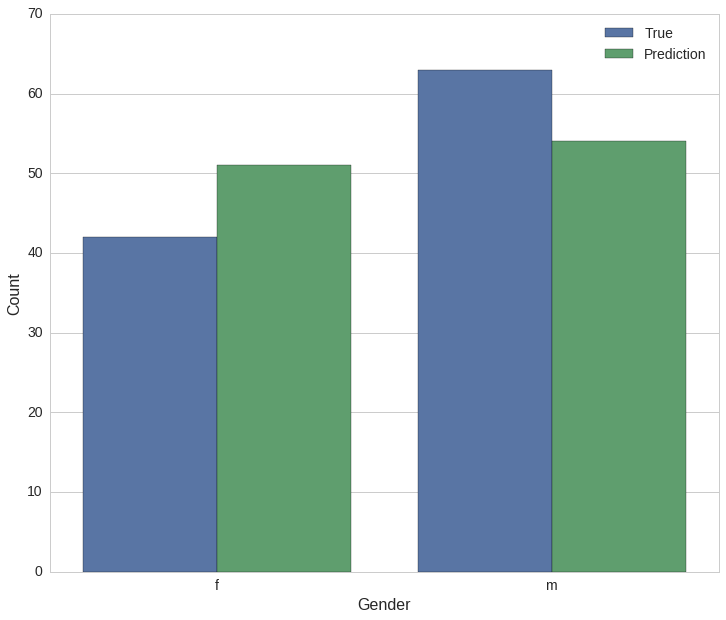
\includegraphics[width=\linewidth]{fig/gender_dist.png}
\caption{Distribution of gender predictions and true labels.}
\label{fig:gender_dist}
\end{subfigure}
\hspace{1em}
\begin{subfigure}[b]{0.45\textwidth}
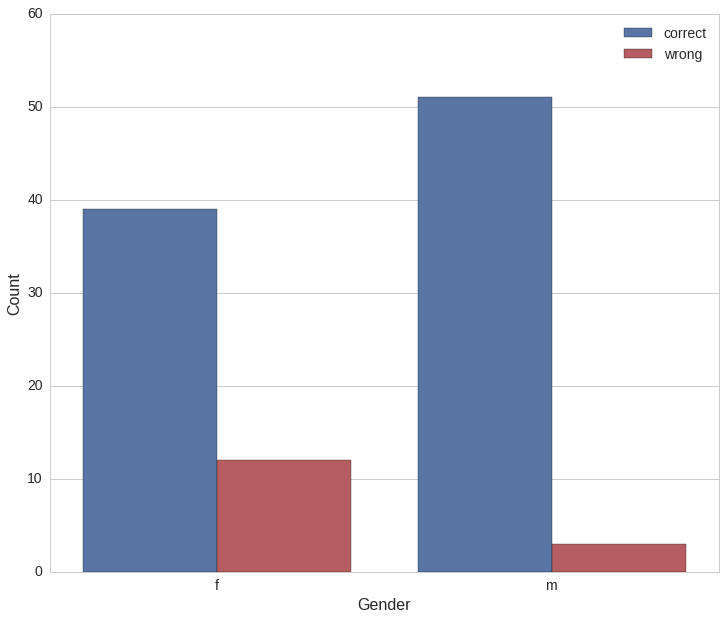
\includegraphics[width=\linewidth]{fig/gender_error.png}
\caption{TP, TN, FP and FN rates for the gender predictions (`f' is said to be positive).}
\label{fig:gender_error}
\end{subfigure}
\caption{Gender predictor metrics.}
\label{fig:gender}
\end{figure}
  


What we're doing here can be considered a no-go, by ML standards. However, since we're using only these `hand-generated' features, and they are designed to adhere to as general standards as possible, the chance of overfitting is minimal. On top of this, we're using the weights generated by the model merely to confirm suspicions that we already had about each feature's importance. 

For example, the score measuring specific pronouns in the window with $c_i$ is error-prone by design. The pronouns `il' and `elle' are among the most frequent words in the French language. The scores of specific titles or articles immediately preceding a $c_i$ occurrence is far more precise, and thus also less prone to error (or noise). It's safe to assume that these last two will have a higher weight than the first. This was confirmed by the weights given by our models. 

As a sanity-check, we generated predictions on some unused books during training of the weights, and verified that results are similar to the ones we obtained in \cref{tab:gender_metrics} . Usually, they were a few percent lower, i.e. for \textit{Nana}, by Zola (66 characters), we get an accuracy of $82.1\%$, precision, recall and f-score of $75.8\%, 88\%, 81.5\%$ respectively and a known ratio of $0.848$.

By the nature of our features (specific word types or words occurring in window with $c_i$), about $20\%$ of data points remain undecided (neutral). A quick look at these characters indicates that none of these play a major role within the book, so we can assume this is due to a lack of data.

\begin{figure}
\centering
  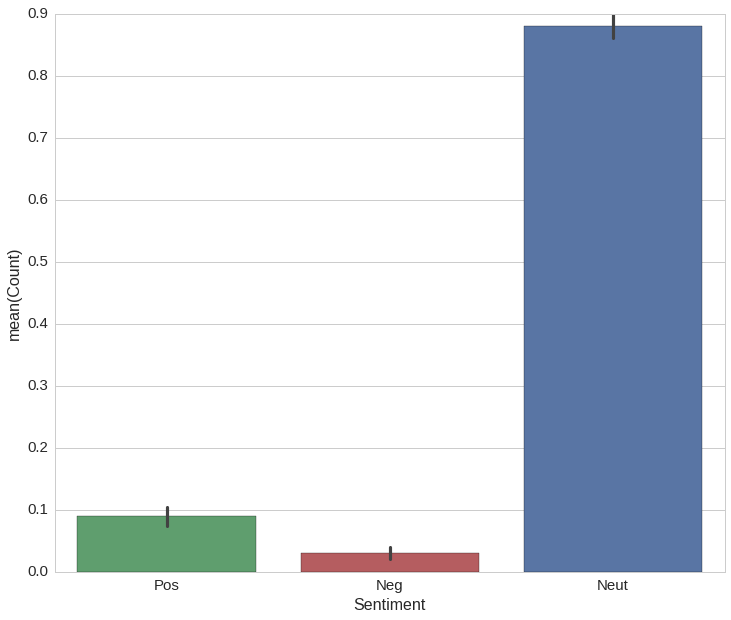
\includegraphics[width=0.6\textwidth]{fig/sent_prop.png}
  \caption{Mean proportions of positive, negative and neutral sentences for reduced character documents. Here the mean for all characters are shown.}
  \label{fig:sent_prop}
\end{figure}

\subsection{Sentiment predictor}
The results of the sentiment predictor on the characters is meaningful mainly for major characters. The API used returns the result `neutral' for most sentences it receives (c.f. \cref{fig:sent_prop}. So for a small number of sentences, we will have only a handful that indicate any sentiment, according to the NLTK tool we use. This may be due to a justifiably conservative predicting scheme on the part of the text classifier, however it has as a consequence that we're unable to extract a truthful understanding around the sentiment pertaining to a character in a novel, which is often associated with hundreds of sentences, and a wide range of polar descriptions.

Some characters with obvious polarities associated with them (i.e. Mrs Aouada, from \textit{Le Tour du Monde en 80 Jours} should be positive, Hutin from \textit{Au Bonheur des Dames} should be negative), are predicted with the wrong or no polarity (c.f. \cref{tab:full_vs_red}). 

With additional resources, less limited access to the NLTK text sentiment classification API, we could have compromised less. In order to truly evaluate such a result, as we did for the `gender' predictor, we would need access to expert-reviewed labels for a set of books. Associated sentiment is too ambiguous a notion for us to make a decision about the less than obvious characters. We also didn't intend for this predictor to answer a precise question about a character's sentiment throughout a narrative, but rather to understand sentiment associated with a character like a bubble surrounding his or her actions. 

\begin{table}
\centering
\begin{tabular}{| l | l || *{4}{c|}}
\hline
& Doc size & Pos-ratio & Neg-ratio	& Neut-ratio & Total count	\\ \hline \hline
\multirow{2}{*}{Denise} & reduced & 0.059 & 0.059 & \bf 0.882 & 51 \\ \cline{2-6}
& full & \bf 0.074 & 0.049 & 0.877	& 511 	\\ \hline

\multirow{2}{*}{Hutin} & reduced	& 0.0	& 0.0	& \bf 1.00	& 12 \\ \cline{2-6}
	& full & 0.032 & 0.032 & \bf 0.935	&  124	\\ \hline
    
\multirow{2}{*}{Bourdoncle}	& reduced & 0.0	& 0.0	& \bf 1.0	& 11 \\ \cline{2-6}
	& full & \bf 0.085 & 0.043 & 0.872 & 117 \\ \hline
    
\multirow{2}{*}{MrsAouda} & reduced	& 0.083	& \bf 0.167	&  0.88 & 12 \\ \cline{2-6}
	& full & \bf 0.062 & 0.039 & 0.899	& 129 	\\ \hline

\end{tabular}
\caption{Performance of the sentiment predictor on some main characters. A character is said to be positive if it has a higher ratio than the negative, and vice-versa.}
\label{tab:full_vs_red}
\end{table}

\vspace{3em}

%%%% PLOT MEAN JOB PREDICTIONS FOR PHILEASFOGG MFOGG AND FOGG AND THEN ALL THREE AGGREGATED > COST OF AMBIGUITY